Marine oil spill is a form of human made environmental pollution that usually occurs during transportation of oil, extracting oil with drilling platforms \cite{Zhang201476} or during the maintenance on oil exploration sites in the ocean. One of the largest occurrences of oil spills in history happened in the Gulf of Mexico, the oil spread out in the ocean caused by the explosion on the drilling platform affected marine ecosystem and wild life\cite{Bozeman2011244}. The New York Times wrote about the aftermath \cite{bpnytimes}. In their article they discuss the massive financial consequences for the oil company BP, as they ended up paying 27 billion dollars to clean up the oil.

Detection of oil spills can help to control environmental risks and prevent damages. Synthetic aperture radar(SAR) images are useful to detect oil spills spots in the ocean. \\
There are various automated systems in order to detect spills spots in SAR images. These systems analyze the SAR images, identify possible oil spills and use an algorithm to classify it as either an oil spill or lookalike \cite{Xu201414,brekke2008classifiers,Keramitsoglou2006640,Guo2014146}. Lookalikes are natural phenomena that appear as a dark spot as well in SAR images. These include algea, seaweed infestations, grease ice, rain cells and low wind condition. This paper is about studying which classification method leads to the highest accuracy in successful discrimination between oil spills and lookalikes.

An overview of a general oil spill detection process is presented in figure \ref{fig:oilspillapproach}, this paper will follow the same strategy. We will start this article by looking at different imaging methods used in oil spill detection, but we will focus on SAR. Afterwards, we will examine the preprocessing of SAR images. Thirdly, an explanation of the features used in oil spill detection is given. We shortly touch on how they are extracted and why these are commonly used. We then quickly explain the three different supervised learning classification methods we want to compare. In section four we compare our three classifiers with each other. Next, we'll have a discussion based on the results of section four. Here we look at which classifier is a good choice for oil spill detection. We finalize our paper with a conclusion and recommendations.

\begin{figure}[H]
	\centering
    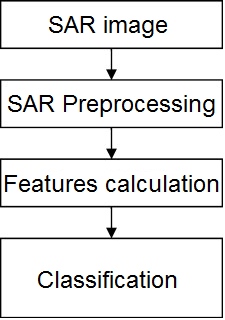
\includegraphics[width=30mm,scale=0.2]{./img/basicsteps.png}
    \caption{\footnotesize{Overview for the oil spill detection approach}}
    \label{fig:oilspillapproach}
\end{figure}